\subsection{Modelo em CAD dos componentes da turbina}

Através da plataforma Solidworks, foram modelados elementos da turbina
necessários para a simulação. Após modelagem, os componentes são importados no
OpenRAVE no formato .wrl: aro câmara, rotor, íris, pá do rotor, e robô MH12 da
Motoman, objeto de estudo da simulação (figura~\ref{fig::arocamara}).

\begin{figure}[!ht]
	\centering	
	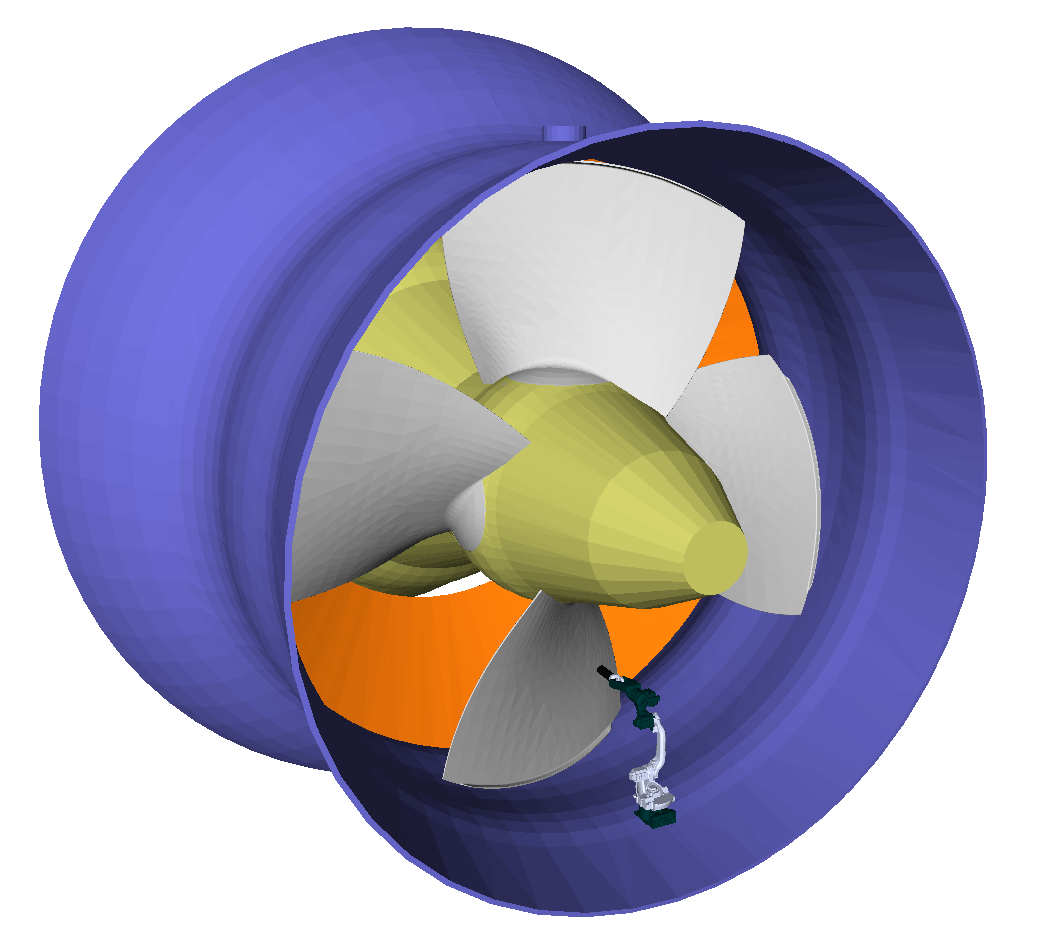
\includegraphics[width=.5\columnwidth]{figs/arocamara.png}
	\caption{Modelo CAD dos componentes da turbina e robô.}
	\label{fig::arocamara}
\end{figure}